% Options for packages loaded elsewhere
% Options for packages loaded elsewhere
\PassOptionsToPackage{unicode}{hyperref}
\PassOptionsToPackage{hyphens}{url}
\PassOptionsToPackage{dvipsnames,svgnames,x11names}{xcolor}
%
\documentclass[
  letterpaper,
  DIV=11,
  numbers=noendperiod]{scrartcl}
\usepackage{xcolor}
\usepackage{amsmath,amssymb}
\setcounter{secnumdepth}{-\maxdimen} % remove section numbering
\usepackage{iftex}
\ifPDFTeX
  \usepackage[T1]{fontenc}
  \usepackage[utf8]{inputenc}
  \usepackage{textcomp} % provide euro and other symbols
\else % if luatex or xetex
  \usepackage{unicode-math} % this also loads fontspec
  \defaultfontfeatures{Scale=MatchLowercase}
  \defaultfontfeatures[\rmfamily]{Ligatures=TeX,Scale=1}
\fi
\usepackage{lmodern}
\ifPDFTeX\else
  % xetex/luatex font selection
\fi
% Use upquote if available, for straight quotes in verbatim environments
\IfFileExists{upquote.sty}{\usepackage{upquote}}{}
\IfFileExists{microtype.sty}{% use microtype if available
  \usepackage[]{microtype}
  \UseMicrotypeSet[protrusion]{basicmath} % disable protrusion for tt fonts
}{}
\makeatletter
\@ifundefined{KOMAClassName}{% if non-KOMA class
  \IfFileExists{parskip.sty}{%
    \usepackage{parskip}
  }{% else
    \setlength{\parindent}{0pt}
    \setlength{\parskip}{6pt plus 2pt minus 1pt}}
}{% if KOMA class
  \KOMAoptions{parskip=half}}
\makeatother
% Make \paragraph and \subparagraph free-standing
\makeatletter
\ifx\paragraph\undefined\else
  \let\oldparagraph\paragraph
  \renewcommand{\paragraph}{
    \@ifstar
      \xxxParagraphStar
      \xxxParagraphNoStar
  }
  \newcommand{\xxxParagraphStar}[1]{\oldparagraph*{#1}\mbox{}}
  \newcommand{\xxxParagraphNoStar}[1]{\oldparagraph{#1}\mbox{}}
\fi
\ifx\subparagraph\undefined\else
  \let\oldsubparagraph\subparagraph
  \renewcommand{\subparagraph}{
    \@ifstar
      \xxxSubParagraphStar
      \xxxSubParagraphNoStar
  }
  \newcommand{\xxxSubParagraphStar}[1]{\oldsubparagraph*{#1}\mbox{}}
  \newcommand{\xxxSubParagraphNoStar}[1]{\oldsubparagraph{#1}\mbox{}}
\fi
\makeatother

\usepackage{color}
\usepackage{fancyvrb}
\newcommand{\VerbBar}{|}
\newcommand{\VERB}{\Verb[commandchars=\\\{\}]}
\DefineVerbatimEnvironment{Highlighting}{Verbatim}{commandchars=\\\{\}}
% Add ',fontsize=\small' for more characters per line
\usepackage{framed}
\definecolor{shadecolor}{RGB}{241,243,245}
\newenvironment{Shaded}{\begin{snugshade}}{\end{snugshade}}
\newcommand{\AlertTok}[1]{\textcolor[rgb]{0.68,0.00,0.00}{#1}}
\newcommand{\AnnotationTok}[1]{\textcolor[rgb]{0.37,0.37,0.37}{#1}}
\newcommand{\AttributeTok}[1]{\textcolor[rgb]{0.40,0.45,0.13}{#1}}
\newcommand{\BaseNTok}[1]{\textcolor[rgb]{0.68,0.00,0.00}{#1}}
\newcommand{\BuiltInTok}[1]{\textcolor[rgb]{0.00,0.23,0.31}{#1}}
\newcommand{\CharTok}[1]{\textcolor[rgb]{0.13,0.47,0.30}{#1}}
\newcommand{\CommentTok}[1]{\textcolor[rgb]{0.37,0.37,0.37}{#1}}
\newcommand{\CommentVarTok}[1]{\textcolor[rgb]{0.37,0.37,0.37}{\textit{#1}}}
\newcommand{\ConstantTok}[1]{\textcolor[rgb]{0.56,0.35,0.01}{#1}}
\newcommand{\ControlFlowTok}[1]{\textcolor[rgb]{0.00,0.23,0.31}{\textbf{#1}}}
\newcommand{\DataTypeTok}[1]{\textcolor[rgb]{0.68,0.00,0.00}{#1}}
\newcommand{\DecValTok}[1]{\textcolor[rgb]{0.68,0.00,0.00}{#1}}
\newcommand{\DocumentationTok}[1]{\textcolor[rgb]{0.37,0.37,0.37}{\textit{#1}}}
\newcommand{\ErrorTok}[1]{\textcolor[rgb]{0.68,0.00,0.00}{#1}}
\newcommand{\ExtensionTok}[1]{\textcolor[rgb]{0.00,0.23,0.31}{#1}}
\newcommand{\FloatTok}[1]{\textcolor[rgb]{0.68,0.00,0.00}{#1}}
\newcommand{\FunctionTok}[1]{\textcolor[rgb]{0.28,0.35,0.67}{#1}}
\newcommand{\ImportTok}[1]{\textcolor[rgb]{0.00,0.46,0.62}{#1}}
\newcommand{\InformationTok}[1]{\textcolor[rgb]{0.37,0.37,0.37}{#1}}
\newcommand{\KeywordTok}[1]{\textcolor[rgb]{0.00,0.23,0.31}{\textbf{#1}}}
\newcommand{\NormalTok}[1]{\textcolor[rgb]{0.00,0.23,0.31}{#1}}
\newcommand{\OperatorTok}[1]{\textcolor[rgb]{0.37,0.37,0.37}{#1}}
\newcommand{\OtherTok}[1]{\textcolor[rgb]{0.00,0.23,0.31}{#1}}
\newcommand{\PreprocessorTok}[1]{\textcolor[rgb]{0.68,0.00,0.00}{#1}}
\newcommand{\RegionMarkerTok}[1]{\textcolor[rgb]{0.00,0.23,0.31}{#1}}
\newcommand{\SpecialCharTok}[1]{\textcolor[rgb]{0.37,0.37,0.37}{#1}}
\newcommand{\SpecialStringTok}[1]{\textcolor[rgb]{0.13,0.47,0.30}{#1}}
\newcommand{\StringTok}[1]{\textcolor[rgb]{0.13,0.47,0.30}{#1}}
\newcommand{\VariableTok}[1]{\textcolor[rgb]{0.07,0.07,0.07}{#1}}
\newcommand{\VerbatimStringTok}[1]{\textcolor[rgb]{0.13,0.47,0.30}{#1}}
\newcommand{\WarningTok}[1]{\textcolor[rgb]{0.37,0.37,0.37}{\textit{#1}}}

\usepackage{longtable,booktabs,array}
\newcounter{none} % for unnumbered tables
\usepackage{calc} % for calculating minipage widths
% Correct order of tables after \paragraph or \subparagraph
\usepackage{etoolbox}
\makeatletter
\patchcmd\longtable{\par}{\if@noskipsec\mbox{}\fi\par}{}{}
\makeatother
% Allow footnotes in longtable head/foot
\IfFileExists{footnotehyper.sty}{\usepackage{footnotehyper}}{\usepackage{footnote}}
\makesavenoteenv{longtable}
\usepackage{graphicx}
\makeatletter
\newsavebox\pandoc@box
\newcommand*\pandocbounded[1]{% scales image to fit in text height/width
  \sbox\pandoc@box{#1}%
  \Gscale@div\@tempa{\textheight}{\dimexpr\ht\pandoc@box+\dp\pandoc@box\relax}%
  \Gscale@div\@tempb{\linewidth}{\wd\pandoc@box}%
  \ifdim\@tempb\p@<\@tempa\p@\let\@tempa\@tempb\fi% select the smaller of both
  \ifdim\@tempa\p@<\p@\scalebox{\@tempa}{\usebox\pandoc@box}%
  \else\usebox{\pandoc@box}%
  \fi%
}
% Set default figure placement to htbp
\def\fps@figure{htbp}
\makeatother





\setlength{\emergencystretch}{3em} % prevent overfull lines

\providecommand{\tightlist}{%
  \setlength{\itemsep}{0pt}\setlength{\parskip}{0pt}}



 


\usepackage{booktabs}
\usepackage{longtable}
\usepackage{array}
\usepackage{multirow}
\usepackage{wrapfig}
\usepackage{float}
\usepackage{colortbl}
\usepackage{pdflscape}
\usepackage{tabu}
\usepackage{threeparttable}
\usepackage{threeparttablex}
\usepackage[normalem]{ulem}
\usepackage{makecell}
\usepackage{xcolor}
\KOMAoption{captions}{tableheading}
\makeatletter
\@ifpackageloaded{tcolorbox}{}{\usepackage[skins,breakable]{tcolorbox}}
\@ifpackageloaded{fontawesome5}{}{\usepackage{fontawesome5}}
\definecolor{quarto-callout-color}{HTML}{909090}
\definecolor{quarto-callout-note-color}{HTML}{0758E5}
\definecolor{quarto-callout-important-color}{HTML}{CC1914}
\definecolor{quarto-callout-warning-color}{HTML}{EB9113}
\definecolor{quarto-callout-tip-color}{HTML}{00A047}
\definecolor{quarto-callout-caution-color}{HTML}{FC5300}
\definecolor{quarto-callout-color-frame}{HTML}{acacac}
\definecolor{quarto-callout-note-color-frame}{HTML}{4582ec}
\definecolor{quarto-callout-important-color-frame}{HTML}{d9534f}
\definecolor{quarto-callout-warning-color-frame}{HTML}{f0ad4e}
\definecolor{quarto-callout-tip-color-frame}{HTML}{02b875}
\definecolor{quarto-callout-caution-color-frame}{HTML}{fd7e14}
\makeatother
\makeatletter
\@ifpackageloaded{caption}{}{\usepackage{caption}}
\AtBeginDocument{%
\ifdefined\contentsname
  \renewcommand*\contentsname{Table of contents}
\else
  \newcommand\contentsname{Table of contents}
\fi
\ifdefined\listfigurename
  \renewcommand*\listfigurename{List of Figures}
\else
  \newcommand\listfigurename{List of Figures}
\fi
\ifdefined\listtablename
  \renewcommand*\listtablename{List of Tables}
\else
  \newcommand\listtablename{List of Tables}
\fi
\ifdefined\figurename
  \renewcommand*\figurename{Figure}
\else
  \newcommand\figurename{Figure}
\fi
\ifdefined\tablename
  \renewcommand*\tablename{Table}
\else
  \newcommand\tablename{Table}
\fi
}
\@ifpackageloaded{float}{}{\usepackage{float}}
\floatstyle{ruled}
\@ifundefined{c@chapter}{\newfloat{codelisting}{h}{lop}}{\newfloat{codelisting}{h}{lop}[chapter]}
\floatname{codelisting}{Listing}
\newcommand*\listoflistings{\listof{codelisting}{List of Listings}}
\makeatother
\makeatletter
\makeatother
\makeatletter
\@ifpackageloaded{caption}{}{\usepackage{caption}}
\@ifpackageloaded{subcaption}{}{\usepackage{subcaption}}
\makeatother
\usepackage{bookmark}
\IfFileExists{xurl.sty}{\usepackage{xurl}}{} % add URL line breaks if available
\urlstyle{same}
\hypersetup{
  pdftitle={Lab 8: Multiple Regression},
  colorlinks=true,
  linkcolor={blue},
  filecolor={Maroon},
  citecolor={Blue},
  urlcolor={Blue},
  pdfcreator={LaTeX via pandoc}}


\title{Lab 8: Multiple Regression}
\author{}
\date{}
\begin{document}
\maketitle


Due: Friday, Apr 17, 2026 at 11:59PM

\subsection{Set up}\label{set-up}

\begin{enumerate}
\def\labelenumi{\arabic{enumi}.}
\item
  \textbf{Open your RStudio project} by going to File \textgreater{}
  Open Project. Select your BIOS 600 folder. (If you see a blue cube
  with your project name at the top right of your RStudio window, you're
  good to go - you are already in your project folder.)
\item
  To begin, start a new Quarto file. Change the title to Lab 8. Keep the
  output as html.
\item
  ``Save As'' into your class project folder with a new name:
  ``\texttt{lab-08.qmd}''.
\item
  Update your name and date in the YAML.
\item
  Render your document to make sure your YAML is rendering correctly.
\end{enumerate}

\begin{tcolorbox}[enhanced jigsaw, arc=.35mm, bottomrule=.15mm, bottomtitle=1mm, breakable, colback=white, colbacktitle=quarto-callout-tip-color!10!white, colframe=quarto-callout-tip-color-frame, coltitle=black, left=2mm, leftrule=.75mm, opacityback=0, opacitybacktitle=0.6, rightrule=.15mm, title=\textcolor{quarto-callout-tip-color}{\faLightbulb}\hspace{0.5em}{Data download}, titlerule=0mm, toprule=.15mm, toptitle=1mm]

Download \texttt{cdc.csv} and \texttt{beijing.csv} and save into your
Data folder within your BIOS 600 Project folder.

\end{tcolorbox}

\subsection{Loading libraries}\label{loading-libraries}

Below you'll find the packages needed for today's lab. You may need to
use \texttt{install.packages} first.

\begin{Shaded}
\begin{Highlighting}[]
\FunctionTok{library}\NormalTok{(tidyverse)}
\FunctionTok{library}\NormalTok{(broom)}
\FunctionTok{library}\NormalTok{(kableExtra)}
\end{Highlighting}
\end{Shaded}

\subsection{Fitting linear models}\label{fitting-linear-models}

In R, we use the \texttt{lm()} function to fit linear models. It is
often useful to save the ``model object'' as a separate object in order
to use it for downstream analyses. In general, the syntax is

\begin{Shaded}
\begin{Highlighting}[]
\NormalTok{model }\OtherTok{\textless{}{-}} \FunctionTok{lm}\NormalTok{(outcome }\SpecialCharTok{\textasciitilde{}}\NormalTok{ predictor1 }\SpecialCharTok{+}\NormalTok{ predictor2 }\SpecialCharTok{+}\NormalTok{ ..., }\AttributeTok{data =}\NormalTok{ dataset)}
\end{Highlighting}
\end{Shaded}

Let's read in the \texttt{cdc} data.

\begin{Shaded}
\begin{Highlighting}[]
\NormalTok{cdc }\OtherTok{\textless{}{-}} \FunctionTok{read.csv}\NormalTok{(}\StringTok{"data/cdc.csv"}\NormalTok{)}
\end{Highlighting}
\end{Shaded}

Now let's fit a linear model using the CDC data, where our response
variable is obesity percentage and the three predictor variables are
adequate exercise percentage, smoking percentage, and HDI category, and
suppose we want to save it as the object \texttt{mod1}. We would use the
following code:

\begin{Shaded}
\begin{Highlighting}[]
\NormalTok{mod1 }\OtherTok{\textless{}{-}} \FunctionTok{lm}\NormalTok{(Obesity }\SpecialCharTok{\textasciitilde{}}\NormalTok{ Exercise }\SpecialCharTok{+}\NormalTok{ Smoking }\SpecialCharTok{+}\NormalTok{ HDI, }\AttributeTok{data =}\NormalTok{ cdc)}
\end{Highlighting}
\end{Shaded}

\subsection{Model estimates}\label{model-estimates}

First, let's take a look at the model output with the \texttt{tidy}
function. This function is applied to a linear model object such as the
mod1 object we saved earlier:

\begin{Shaded}
\begin{Highlighting}[]
\FunctionTok{tidy}\NormalTok{(mod1)}
\end{Highlighting}
\end{Shaded}

\begin{verbatim}
# A tibble: 5 x 5
  term        estimate std.error statistic  p.value
  <chr>          <dbl>     <dbl>     <dbl>    <dbl>
1 (Intercept)   37.6      3.57      10.5   9.66e-14
2 Exercise      -0.281    0.0539    -5.22  4.46e- 6
3 Smoking        0.431    0.0922     4.68  2.68e- 5
4 HDIMiddle     -0.724    0.794     -0.912 3.67e- 1
5 HDITop ten    -2.78     1.00      -2.77  8.07e- 3
\end{verbatim}

We see that the output provides columns containing our coefficient
estimates, their standard errors, the t-statistic corresponding to each,
and the p-value.

Note that R automatically recognized \texttt{HDI} as a categorical
variable since its values are character strings, and created the
appropriate dummy variables (treating the first category in alphabetical
order as the baseline value). If you have a categorical variable that
takes on numerical values, you can use the \texttt{as.factor} function
in the model call to convert a variable into a categorical variable
(which R will create dummy variables from). For instance:

\begin{Shaded}
\begin{Highlighting}[]
\NormalTok{model }\OtherTok{\textless{}{-}} \FunctionTok{lm}\NormalTok{(outcome }\SpecialCharTok{+}\NormalTok{ predictor1 }\SpecialCharTok{+} \FunctionTok{as.factor}\NormalTok{(predictor2) }\SpecialCharTok{+}\NormalTok{ ..., }\AttributeTok{data =}\NormalTok{ dataset)}
\end{Highlighting}
\end{Shaded}

As well, we can get model-specific values such as the \(R^2\), adjusted
\(R^2\), the F-statistic (and corresponding p-value), and some other
statistics by using the \texttt{glance} function applied to our model
object. Note that the \texttt{df} given in the table is the numerator
degrees of freedom for the overall F test.

\begin{Shaded}
\begin{Highlighting}[]
\FunctionTok{glance}\NormalTok{(mod1)}
\end{Highlighting}
\end{Shaded}

\begin{verbatim}
# A tibble: 1 x 12
  r.squared adj.r.squared sigma statistic  p.value    df logLik   AIC   BIC
      <dbl>         <dbl> <dbl>     <dbl>    <dbl> <dbl>  <dbl> <dbl> <dbl>
1     0.805         0.787  1.67      46.3 2.11e-15     4  -94.1  200.  212.
# i 3 more variables: deviance <dbl>, df.residual <int>, nobs <int>
\end{verbatim}

\subsection{Evaluating residuals}\label{evaluating-residuals}

The \texttt{augment()} function from the \texttt{broom} package gives us
some additional information relating to our linear model. Of primary
interest are the fitted values and the residuals for each observation.
The fitted values are the predicted response values given the values for
our explanatory variables, and the residuals are the difference between
the actual response data points and their fitted (predicted) values from
the model.

Let's apply the augment function to the mod1 object we created earlier,
and save it as a new dataframe, \texttt{mod1\_res} (which contains the
residuals):

\begin{Shaded}
\begin{Highlighting}[]
\NormalTok{mod1\_res }\OtherTok{\textless{}{-}} \FunctionTok{augment}\NormalTok{(mod1)}
\end{Highlighting}
\end{Shaded}

The variables \texttt{.fitted} and \texttt{.resid} (note the period)
variables from this dataframe are what we will be using to evaluate some
model assumptions. For instance, we could evaluate the normality of the
residuals by plotting a histogram, or evaluate linearity/homogeneity of
variances by plotting a scatterplot of the fitted values vs.~the
residuals.

For instance, we can create a ggplot histogram of the .resid to get a
histogram of the residuals:

\begin{Shaded}
\begin{Highlighting}[]
\FunctionTok{ggplot}\NormalTok{(}\AttributeTok{data =}\NormalTok{ mod1\_res, }\AttributeTok{mapping =} \FunctionTok{aes}\NormalTok{(}\AttributeTok{x =}\NormalTok{ .resid)) }\SpecialCharTok{+} 
  \FunctionTok{geom\_histogram}\NormalTok{(}\AttributeTok{binwidth =} \DecValTok{1}\NormalTok{) }\SpecialCharTok{+} 
  \FunctionTok{labs}\NormalTok{(}\AttributeTok{x =} \StringTok{"Residuals"}\NormalTok{, }\AttributeTok{y =} \StringTok{"Count"}\NormalTok{,}
       \AttributeTok{title =} \StringTok{"Residuals are slightly right{-}skewed"}\NormalTok{)}
\end{Highlighting}
\end{Shaded}

\pandocbounded{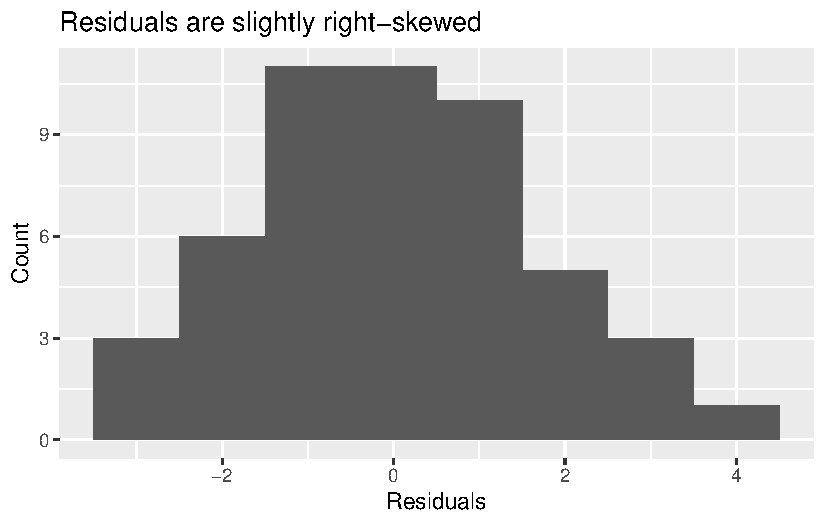
\includegraphics[keepaspectratio]{lab-08_AGH_files/figure-pdf/unnamed-chunk-9-1.pdf}}

Or a scatterplot of the fitted values vs.~the residuals (the residual
plot):

\begin{Shaded}
\begin{Highlighting}[]
\FunctionTok{ggplot}\NormalTok{(}\AttributeTok{data =}\NormalTok{ mod1\_res, }\AttributeTok{mapping =} \FunctionTok{aes}\NormalTok{(}\AttributeTok{x =}\NormalTok{ .fitted, }\AttributeTok{y =}\NormalTok{ .resid)) }\SpecialCharTok{+} 
  \FunctionTok{geom\_point}\NormalTok{() }\SpecialCharTok{+} 
  \FunctionTok{labs}\NormalTok{(}\AttributeTok{x =} \StringTok{"Fitted values"}\NormalTok{, }\AttributeTok{y =} \StringTok{"Residuals"}\NormalTok{,}
       \AttributeTok{title =} \StringTok{"Residual plot shows no clear pattern"}\NormalTok{)}
\end{Highlighting}
\end{Shaded}

\pandocbounded{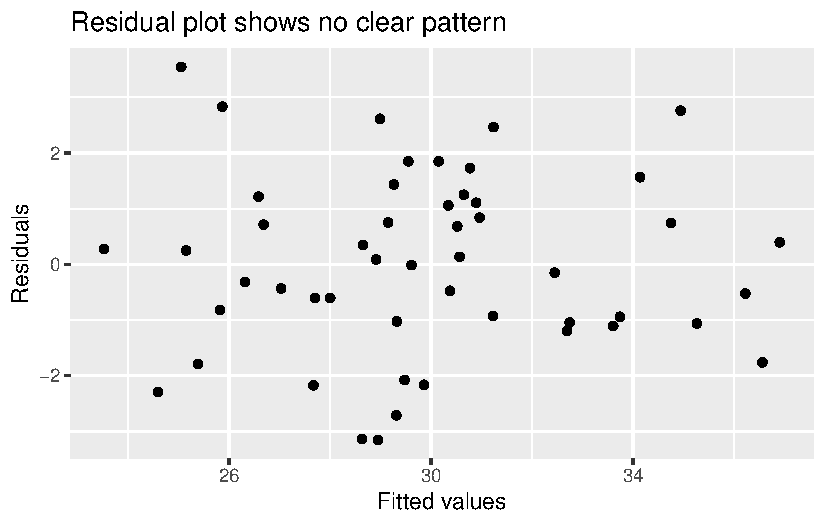
\includegraphics[keepaspectratio]{lab-08_AGH_files/figure-pdf/unnamed-chunk-10-1.pdf}}

\subsection{Predicting new values}\label{predicting-new-values}

We can use our fitted values from our model to predict a new Obesity
percent, given certain values of our predictors.

\begin{Shaded}
\begin{Highlighting}[]
\NormalTok{new\_obs }\OtherTok{\textless{}{-}} \FunctionTok{data.frame}\NormalTok{(}
  \AttributeTok{Exercise =} \DecValTok{45}\NormalTok{,}
  \AttributeTok{Smoking  =} \DecValTok{18}\NormalTok{,}
  \AttributeTok{HDI      =} \StringTok{"Top ten"}\NormalTok{)}

\CommentTok{\# Predicted value with confidence interval}
\FunctionTok{predict}\NormalTok{(mod1, }\AttributeTok{newdata =}\NormalTok{ new\_obs, }
        \AttributeTok{interval =} \StringTok{"confidence"}\NormalTok{)}
\end{Highlighting}
\end{Shaded}

\begin{verbatim}
       fit     lwr      upr
1 29.95768 28.5452 31.37017
\end{verbatim}

\textbf{Conclusion}: Given a region with \texttt{Exercise} = 45\%,
\texttt{Smoking} = 18\%, and given the region is in the Top ten HDI
category, our model predicts an Obesity percentage of 29.957\%.

\subsection{Interactions}\label{interactions}

Interactions in models are made by simplifying multiplying two variables
of interest together. As an example:

\begin{Shaded}
\begin{Highlighting}[]
\NormalTok{mod\_int }\OtherTok{\textless{}{-}} \FunctionTok{lm}\NormalTok{(outcome }\SpecialCharTok{\textasciitilde{}}\NormalTok{ var1 }\SpecialCharTok{+}\NormalTok{ var2 }\SpecialCharTok{+}\NormalTok{ var1 }\SpecialCharTok{*}\NormalTok{ var2, }\AttributeTok{data =}\NormalTok{ dataset)}
\end{Highlighting}
\end{Shaded}

Note the \texttt{var1*var2} term in the model above.

\subsection{Exercise 1}\label{exercise-1}

Using the \texttt{cdc} dataset, consider the following model:

\[Obesity_i = \beta_0 + \beta_1Exercise_i + \beta_2Smoking_i + \beta_3(HDI == Middle)_i + \beta_4 (HDI == Top ten)_i + \epsilon_i\]

\begin{enumerate}
\def\labelenumi{\alph{enumi}.}
\item
  Fit the model using \texttt{lm()}. Display the table of estimated
  regression coefficients using \texttt{tidy()} and \texttt{kable()},
  rounding to 3 digits.
\item
  What is the interpretation of \(\hat \beta_2\)?
\item
  What is the interpretation of \(\hat \beta_4\)?
\end{enumerate}

\subsection{Atmospheric PM2.5}\label{atmospheric-pm2.5}

Atmospheric PM2.5 is fine particulate matter that has a diameter of less
than 2.5 micrometers, and is one of the major air pollutants in the
atmosphere. Such particles penetrate deep into the lungs due to their
small size, and are associated with cardiovascular disease and other
adverse health outcomes. Thus, higher PM2.5 levels imply lower air
quality.

Scientists are interested in evaluating whether atmospheric PM2.5 levels
can be predicted by weather patterns. Hourly data of PM2.5 readings from
2013-2017 were captured at a weather station at Nongzhanguan in Chaoyang
District, Beijing. A modified subset of 1500 of these observations is
given in the \texttt{beijing} dataset, which has been adapted from data
provided by Dr.~Songxi Chen at Peking University (Proc. Roy. Soc. A:
473(2205): 2017.0457 ).

Of interest are the following variables:

\begin{itemize}
\tightlist
\item
  \texttt{PM2.5}: PM10 levels in micrograms per cubic meter
\item
  \texttt{TEMP}: temperature in degrees Celsius
\item
  \texttt{PRES}: barometric pressure in in hPa
\item
  \texttt{DEWP}: dew point in degrees Celsius
\item
  \texttt{RAIN}: hourly precipitation levels in mm
\item
  \texttt{wd}: wind direction (eight compass points)
\end{itemize}

You may read in the data with the following code.

\begin{Shaded}
\begin{Highlighting}[]
\NormalTok{beijing }\OtherTok{\textless{}{-}} \FunctionTok{read.csv}\NormalTok{(}\AttributeTok{file =} \StringTok{"data/beijing.csv"}\NormalTok{)}
\end{Highlighting}
\end{Shaded}

\subsection{Exercise 2}\label{exercise-2}

Suppose we are interested in fitting a linear model that predicts PM2.5
levels based on the temperature, pressure, dew point, precipitation, and
wind direction.

\begin{enumerate}
\def\labelenumi{\alph{enumi}.}
\item
  Using the \texttt{beijing.csv} dataset, run the model using
  \texttt{lm()}. Save it as a model object (choose a sensible name for
  the model object, like \texttt{fit1} or \texttt{mod1}, etc.) You may
  have to write your model on multiple lines for it to fit on the page
  -- please check before submitting!
\item
  Use the \texttt{augment()} function to produce a new data frame which
  contains \texttt{.fitted} and \texttt{.resid}.
\item
  Based on the data frame created in part (b), create a visualization of
  the fitted values vs.~the residuals using \texttt{ggplot()}.
\item
  Based on the plot from part (c), comment on the following: Does the
  equal variance assumption seem to be satisfied? Does the linearity
  assumption seem to be satisfied?
\item
  Based on the data frame created in part (b), produce a histogram of
  the residuals using \texttt{ggplot()}. Does the normality assumption
  seem to be satisfied?
\end{enumerate}

\subsection{Exercise 3}\label{exercise-3}

Based on the model fit in Exercise 2, what PM2.5 level would you predict
for a day with temperature of 11 degrees C, pressure of 1040 hPa, dew
point of 5 degrees C, with no rain and wind coming from the south? To do
this, create a new data frame with the given predictor values, and then
use the \texttt{predict} function.

\begin{tcolorbox}[enhanced jigsaw, arc=.35mm, bottomrule=.15mm, bottomtitle=1mm, breakable, colback=white, colbacktitle=quarto-callout-tip-color!10!white, colframe=quarto-callout-tip-color-frame, coltitle=black, left=2mm, leftrule=.75mm, opacityback=0, opacitybacktitle=0.6, rightrule=.15mm, title=\textcolor{quarto-callout-tip-color}{\faLightbulb}\hspace{0.5em}{Hint}, titlerule=0mm, toprule=.15mm, toptitle=1mm]

To see how the dataset specifies wind direction (i.e.~the character
names of the different levels), use the following code:

\begin{Shaded}
\begin{Highlighting}[]
\FunctionTok{table}\NormalTok{(beijing}\SpecialCharTok{$}\NormalTok{wd)}
\end{Highlighting}
\end{Shaded}

\end{tcolorbox}

\subsection{Exercise 4}\label{exercise-4}

Based on the model fit in Exercise 2, provide the coefficient estimates
and a 1-sentence conclusion for the following values: the intercept, the
slope corresponding to \texttt{TEMP}, and the slope corresponding to
\texttt{wdSW}.

\subsection{Exercise 5}\label{exercise-5}

Regardless of whether the assumptions in Exercise 2 are satisfied, we'd
like to comprehensively evaluate the following question: is there
sufficient evidence that there is a relationship between barometric
pressure and PM2.5 levels, while adjusting for temperature, dew point,
rain, and wind direction? To do so, do the following:

\begin{enumerate}
\def\labelenumi{\alph{enumi}.}
\item
  State your null and alternative hypotheses in words or symbols.
\item
  State the test statistic's distribution under the null hypothesis
  (include name of distribution and degrees of freedom).
\item
  State your p-value and a 1-sentence conclusion. Assume
  \(\alpha = 0.05\).
\end{enumerate}

\begin{tcolorbox}[enhanced jigsaw, arc=.35mm, bottomrule=.15mm, bottomtitle=1mm, breakable, colback=white, colbacktitle=quarto-callout-tip-color!10!white, colframe=quarto-callout-tip-color-frame, coltitle=black, left=2mm, leftrule=.75mm, opacityback=0, opacitybacktitle=0.6, rightrule=.15mm, title=\textcolor{quarto-callout-tip-color}{\faLightbulb}\hspace{0.5em}{Tip}, titlerule=0mm, toprule=.15mm, toptitle=1mm]

\textbf{Note}: the t statistic for a single predictor in a multiple
regression model follows a \(t\)-distribution with \(𝑛−𝑘\) degrees of
freedom, where \(n\) is the number of observations, and \(k\) is the
number of parameters being estimated (including the intercept).

\end{tcolorbox}

\subsection{Exercise 6}\label{exercise-6}

Given the model in Exercise 2:

\begin{enumerate}
\def\labelenumi{\alph{enumi}.}
\item
  What would be the expected difference in PM2.5 levels given a one
  degree increase in dewpoint? (1-sentence)
\item
  Compute the adjusted \(R^2\) value from the model in Exercise 2 using
  \texttt{glance()}. Provide a 1-sentence interpretation of the adjusted
  \(R^2\) value.
\end{enumerate}

\subsection{AI Attestation}\label{ai-attestation}

Was AI used on this assignment? If so, describe your prompts below. If
not, simply state ``AI was not used on this assignment.''

\subsection{Submission}\label{submission}

As you've seen previously, we can \textbf{Render} the template into an
.html file that can be opened by any web browser. To export it as a
.pdf, open the file in your web browser and then print to or save as a
.pdf document. Your TAs will show you how if you need help! (There is a
way to directly knit to a .pdf file, but it's quite a bit more
involved.)

You will submit the PDF documents for labs and homework to Gradescope as
part of your final submission.

To submit your assignment:

\begin{itemize}
\item
  Access Gradescope through the menu on the BIOS 600 Canvas site.
\item
  Click on the assignment, and you'll be prompted to submit it.
\item
  Mark the pages associated with each exercise. All of the pages of your
  lab should be associated with at least one question (i.e., should be
  ``checked'').
\item
  Select the first page of your .PDF submission to be associated with
  the ``Formatting'' section.
\end{itemize}

\subsection{Grading}\label{grading}

{\def\LTcaptype{none} % do not increment counter
\begin{longtable}[]{@{}ll@{}}
\toprule\noalign{}
Component & Points \\
\midrule\noalign{}
\endhead
\bottomrule\noalign{}
\endlastfoot
Ex 1 & 6 \\
Ex 2 & 7 \\
Ex 3 & 2 \\
Ex 4 & 3 \\
Ex 5 & 5 \\
Ex 6 & 2 \\
AI Attestation & 1 \\
Formatting & 3 \\
\end{longtable}
}

The ``Formatting'' grade is to assess the document format. This includes
having a neatly organized document (no excessive output,
warnings/messages when loading packages and/or data) with readable code
and your name and the date updated in the YAML.




\end{document}
